\documentclass[]{article}
\usepackage[T1]{fontenc}
\usepackage{lmodern}
\usepackage{amssymb,amsmath}
\usepackage{ifxetex,ifluatex}
\usepackage{fixltx2e} % provides \textsubscript
% use upquote if available, for straight quotes in verbatim environments
\IfFileExists{upquote.sty}{\usepackage{upquote}}{}
\ifnum 0\ifxetex 1\fi\ifluatex 1\fi=0 % if pdftex
  \usepackage[utf8]{inputenc}
\else % if luatex or xelatex
  \ifxetex
    \usepackage{mathspec}
    \usepackage{xltxtra,xunicode}
  \else
    \usepackage{fontspec}
  \fi
  \defaultfontfeatures{Mapping=tex-text,Scale=MatchLowercase}
  \newcommand{\euro}{€}
\fi
% use microtype if available
\IfFileExists{microtype.sty}{\usepackage{microtype}}{}
\usepackage{longtable,booktabs}
\usepackage{graphicx}
% Redefine \includegraphics so that, unless explicit options are
% given, the image width will not exceed the width of the page.
% Images get their normal width if they fit onto the page, but
% are scaled down if they would overflow the margins.
\makeatletter
\def\ScaleIfNeeded{%
  \ifdim\Gin@nat@width>\linewidth
    \linewidth
  \else
    \Gin@nat@width
  \fi
}
\makeatother
\let\Oldincludegraphics\includegraphics
{%
 \catcode`\@=11\relax%
 \gdef\includegraphics{\@ifnextchar[{\Oldincludegraphics}{\Oldincludegraphics[width=\ScaleIfNeeded]}}%
}%
\ifxetex
  \usepackage[setpagesize=false, % page size defined by xetex
              unicode=false, % unicode breaks when used with xetex
              xetex]{hyperref}
\else
  \usepackage[unicode=true]{hyperref}
\fi
\hypersetup{breaklinks=true,
            bookmarks=true,
            pdfauthor={},
            pdftitle={},
            colorlinks=true,
            citecolor=blue,
            urlcolor=blue,
            linkcolor=magenta,
            pdfborder={0 0 0}}
\urlstyle{same}  % don't use monospace font for urls
\setlength{\parindent}{0pt}
\setlength{\parskip}{6pt plus 2pt minus 1pt}
\setlength{\emergencystretch}{3em}  % prevent overfull lines
\setcounter{secnumdepth}{0}
\usepackage{fancyhdr}
\pagestyle{fancy}
\lhead{C-Lyrics - A Word Cloud for Lyrics}
\rhead{\thepage}
\cfoot{Team 6}
\renewcommand{\headrulewidth}{0.4pt}
\renewcommand{\footrulewidth}{0.4pt}

\title{PaperCloud}
\author{Justine Cocchi\\jcocchi@usc.edu \and Kelsey Fargas\\kfargas@usc.edu \and Mark Krant \\ mkrant@usc.edu\and Milad Gueramian\\gueramia@usc.edu \and Jeff Kang\\kangjr@usc.edu \and Séb Arnold\\arnolds@usc.edu}
\date{20 April 2015}

\title{%
	PaperCloud \\
	\large Second Iteration Report}

\begin{document}

\clearpage\maketitle
\thispagestyle{empty}

\pagebreak

\tableofcontents
\setcounter{tocdepth}{4}
\thispagestyle{empty}

\pagebreak

\section{Executive Summary}\label{executive-summary}

PaperCloud is an internet application on the world wide web, built for
the purpose of organizing words from different researchers' publications
into a word cloud. The publications come exclusively from IEEE and ACM.
This application will allow for the generation of 2 types of clouds and
as such, two types of searches for each cloud. The first is to enter the
full name of the researcher. PaperCloud will then generate a word cloud
(if the input is valid) based on all the MaxWord most common words from
the researcher's papers. The second search option allows the user to
enter a keyword phrase which will result in a wordcloud consisting of
the MaxWords most common words from all the documents searchable (from
the two publications mentioned) containing the keywords. PaperCloud
offers certain other features to simplify further searches and word
cloud generations which are described in the rest of this document.

\section{1 Introduction}\label{introduction}

\subsection{1.1 Purpose}\label{purpose}

The purpose of this document is to clearly describe every aspect of the
second group project for the CSCI-310 course taken at the University of
Southern California in the Spring semester of the year 2015. The
intended audiences of this software requirements specification document
includes, but is not limited to: the members of group six whose names
are listed on the front page of this document and by whom this document
is prepared, the professor of the course Dr.~William G. Halfond, and the
teaching assistant Sonal Mahajan. Other possible audiences include:
students who are at the time of this publication taking the course in
which this project is assigned or any future students of this course who
may read this document should it become available to them by the course
instructor Dr.~William G. Halfond or by any other means which cannot be
predicted at this time. This software development project will hereafter
be referred to as PaperCloud. It is intended for any user with an
internet connection-either through a mobile or stationary platform.

\subsection{1.2 Overview}\label{overview}

This document is to present the management and development structure of
the second iteration of software under construction. The different
processes are explained in detail in the following sections.
Furthermore, the project serves as guide on how to build software using
the SCRUM and Extreme Programming practices of the Agile collection of
processes.

The content regards the two Agile collection development processes
described above. Section 2 elaborates on our use of SCRUM which includes
our project management plan and organization. Section 3 and 4 details
our requirements, design, and implementation planning. Section 5
describes the review process in which we reevaluate the effectiveness of
our strategy and implementation. The Appendix includes some artifacts
and further details on our development process as a whole.

\subsection{1.3 References}\label{references}

{[}1{]} Cunningham, Ward. ``Extreme Programming''. O'Reilly Media. July
2003.

{[}2{]} Wells, Don. ``Extreme Programming''. October 10,2013. April 5,
2015.\url{http://www.extremeprogramming.org/}.

\subsection{1.4 Terminology}\label{terminology}
\begin{longtable}[c]{@{}ll@{}}
\toprule\addlinespace
\begin{minipage}[t]{0.47\columnwidth}\raggedright
Term
\end{minipage} & \begin{minipage}[t]{0.47\columnwidth}\raggedright
Definition
\end{minipage}
\\
\hline
\\\addlinespace
\begin{minipage}[t]{0.47\columnwidth}\raggedright
IEEE
\end{minipage} & \begin{minipage}[t]{0.47\columnwidth}\raggedright
Institute of Electrical and Electronics Engineers
\end{minipage}
\\\addlinespace
\begin{minipage}[t]{0.47\columnwidth}\raggedright
ACM
\end{minipage} & \begin{minipage}[t]{0.47\columnwidth}\raggedright
Association of Computing Machinery
\end{minipage}
\\\addlinespace
\begin{minipage}[t]{0.47\columnwidth}\raggedright
Development team
\end{minipage} & \begin{minipage}[t]{0.47\columnwidth}\raggedright
All of the individuals whose names appear on the cover of this document.
These persons have collectively put this document together and will
collectively implement the software product described in subsequent
sections.
\end{minipage}
\\\addlinespace
\begin{minipage}[t]{0.47\columnwidth}\raggedright
XP
\end{minipage} & \begin{minipage}[t]{0.47\columnwidth}\raggedright
Extreme Programming
\end{minipage}
\\\addlinespace
\begin{minipage}[t]{0.47\columnwidth}\raggedright
Asana
\end{minipage} & \begin{minipage}[t]{0.47\columnwidth}\raggedright
Online planning and time tracking software
\end{minipage}
\\\addlinespace
\begin{minipage}[t]{0.47\columnwidth}\raggedright
arXiv
\end{minipage} & \begin{minipage}[t]{0.47\columnwidth}\raggedright
Application provided by Cornell university that helps with searching for research papers across a wide range of subjects.
\end{minipage}
\\\addlinespace
\begin{minipage}[t]{0.47\columnwidth}\raggedright
Gmail
\end{minipage} & \begin{minipage}[t]{0.47\columnwidth}\raggedright
Email messaging software from Google Inc. Used for communication purposes by development team
\end{minipage}
\\\addlinespace
\begin{minipage}[t]{0.47\columnwidth}\raggedright
Clients/Customers
\end{minipage} & \begin{minipage}[t]{0.47\columnwidth}\raggedright
Professor William G. Halfond and Sonal Mahajan
\end{minipage}
\\\addlinespace
\bottomrule
\end{longtable}



\subsection{1.5 Scope}\label{scope}

PaperCloud is a web based application for generating a horizontally
positioned text word cloud generated from the most commonly occurring
words from a collection of research papers. There are two search options
each correlating to two different clouds that can be generated. In the
first option, the cloud is generated based on the first and last name
search for a particular author. The second search option allows the user
to enter a keyword phrase which results in a word cloud generated based
on words from all articles that contain the keyword phrase.

PaperCloud will be hosted and available to the World Wide Web and will
require no user registration or membership. To access the PaperCloud
service, a user only needs an internet connection and one of the
commonly used web browsers.

\subsection{1.6 Documents}\label{documents}

We used certain third party software products to assists with project
management and implementation. Information for access to these products
can be found below. Asana is used to keep project backlogs and iteration
related scheduling and task completion details for each sprint. Each
member of the development team will chose tasks from the sprint log to
complete and can interact with other members and update information
about task progress on Asana.

For full access to SCRUM meeting notes refer to the Group 6 discussion
board on the course BlackBoard link under the ``Iteration 2 Team
Activity Log'' thread. For a quick reference, refer to the appendix
Section 6.1.

For full access to Asana, the clients are suggested to refer to their
University of Southern California Gmail account where they will find an
invitation to view PaperCloud's Asana account.

For full access to source code, please refer to the project's public
Github page at https://github.com/C-Lyrics/PaperCloud

\section{2 SCRUM Management}\label{scrum-management}

\subsection{2.1 Process Introduction}\label{process-introduction}

The primary purpose of using Scrum is to work together to develop the
product required from the client. In doing so, we broke up the
requirements created in the back log. This way, we were able to
prioritize tasks for the sprint log to better understand which tasks
needed to be completed before others. By building the product in smaller
broken down pieces, the development team was able to give feedback and
changes if necessary.

The Scrum process is comprised of three different procedures: pre-game,
mid-game, and post-game. The pre-game process involves engaging in
planning and high-level design. This included elicitation of the
requirements from the client, and the Scrum sprint cycle. This is
comprised of the delegation of the three main roles, such as Scrum
master, Product owner, and team, and organizing meeting times with the
development team. After clarifying the requirements, the development
team created the product backlog and sprint log. Every member present at
each meeting that occurred answered the workday questions to make sure
the everyone was on track for task completion. The mid-game process
involves developing, wrapping, reviewing, and adjusting. This is
primarily abiding by the sprint logs that were created from the
backlogs. We developed and wrapped code, reviewed code by pair
programming, and make adjustments accordingly. The post-game process
involved closure of the first iteration, which includes the sprint
review and sprint retrospective.

\subsection{2.2 Organisation Planning}\label{organisation-planning}

\subsubsection{2.2.1 Roles}\label{roles}

The group divided the roles in the following manner:

\begin{itemize}
\itemsep1pt\parskip0pt\parsep0pt
\item
  SCRUM Master: Sébastien
\item
  Product Owners: Sonal Mahajan
\item
  Customers: Sonal Mahajan, William Halfond
\item
  Development Team: Sebastien, Mark, Milad, Justine, Jeff, Kelsey
\end{itemize}

Sebastien was chosen by consensus to be our SCRUM master for iteration 2
because he would be available to attend all meetings and he has had
prior experience using SCRUM techniques.

\subsubsection{2.2.2 Teams}\label{teams}

The teams are allocated as the following:

\begin{itemize}
\itemsep1pt\parskip0pt\parsep0pt
\item
  Frontend: Sebastien, Kelsey, Justine
\item
  Backend: Mark, Milad, Jeff
\end{itemize}

These teams were chosen based on the team allocations we used in the
previous iteration, as well as each group member's individual coding
knowledge and experience. We felt that the division of frontend and
backend made sense as we could assign requirements for implementation on
the frontend Javascript and HTML code and the backend PHP code. However,
in order to promote collective code ownership, all team members
partially contributed to the work for both the frontend and the backend.

\subsubsection{2.2.3 Product Backlog and Sprint
Logs}\label{product-backlog-and-sprint-logs}

Asana was used to create a product backlog of project requirements that
were determined based on meetings with the customer. From this product
backlog, we narrowed the list down to a sprint log for our second
iteration of code based on the customer's prioritization of each of the
requirements on the product backlog and our projected ability to
complete these items during the second sprint. The sprint log was
further broken down into implementable tasks that were outlined on
Asana, which allowed us to track the development progress of our second
sprint.

\begin{itemize}
\itemsep1pt\parskip0pt\parsep0pt
\item
  Product Backlog

  \begin{itemize}
  \itemsep1pt\parskip0pt\parsep0pt
  \item
    Search by keyword (ACM and IEEE publications only)
  \item
    Search by researcher (ACM and IEEE publications only)
  \item
    Autocomplete for searching by researcher
  \item
    Ability to see history of searches
  \item
    Click on word in search history generates word cloud from that word
  \item
    Display word cloud with common words from top N pages
  \item
    User selects how many papers included in top N, we decide how to
    order the top N (ex. alphabetical or temporal)
  \item
    Progress bar for progress of generating word cloud
  \item
    Click on word in cloud lets you make new search with that word
  \item
    Click on word in cloud lets you see all research papers with that
    word in it and how frequently the word appears in each one
  \item
    Click on Conference or Journal name creates list of all papers from
    that journal or conference.
  \item
    Display list of research papers that contain selected word in them
    with their authors listed next to them in

    format
  \item
    Click research paper title takes you to a page with a link to
    download the paper
  \item
    Click author name in research paper list takes you to word cloud
    generation of common words from that author's research papers
  \item
    Select research papers to export references in .txt and .pdf format
  \item
    Ability to get BIBTEX reference of each research paper upon hover/
    button press
  \item
    Navigation buttons between all pages
  \end{itemize}
\item
  Sprint Backlog: We have discussed with the customer the tasks to be
  included for our sprint backlog. We requested a prioritized list of
  requirements for the second iteration, and were able to create the
  sprint backlog laid out below at our first scrum meeting for iteration
  2 on April 5th.

  \begin{itemize}
  \itemsep1pt\parskip0pt\parsep0pt
  \item
    Search by keyword (IEEE publications only)
  \item
    Search by researcher (IEEE publications only)
  \item
    Display word cloud from top N research papers (user can't pick N)
  \item
    Progress bar for word cloud generation
  \item
    For the progress bar requirement, we decided that this iteration we
    will not focus on implementing a bar that increments regularly, as
    expected from the requirements, but we will instead deliver a
    progress bar that implements in larger chunks based on key events.
  \item
    Click on word in cloud lets you make new search with that word
  \end{itemize}
\end{itemize}

We expanded on these tasks, as shown in our asana task log. In addition, each sub-task was assigned to a team member.

\begin{figure}[htbp]
\centering
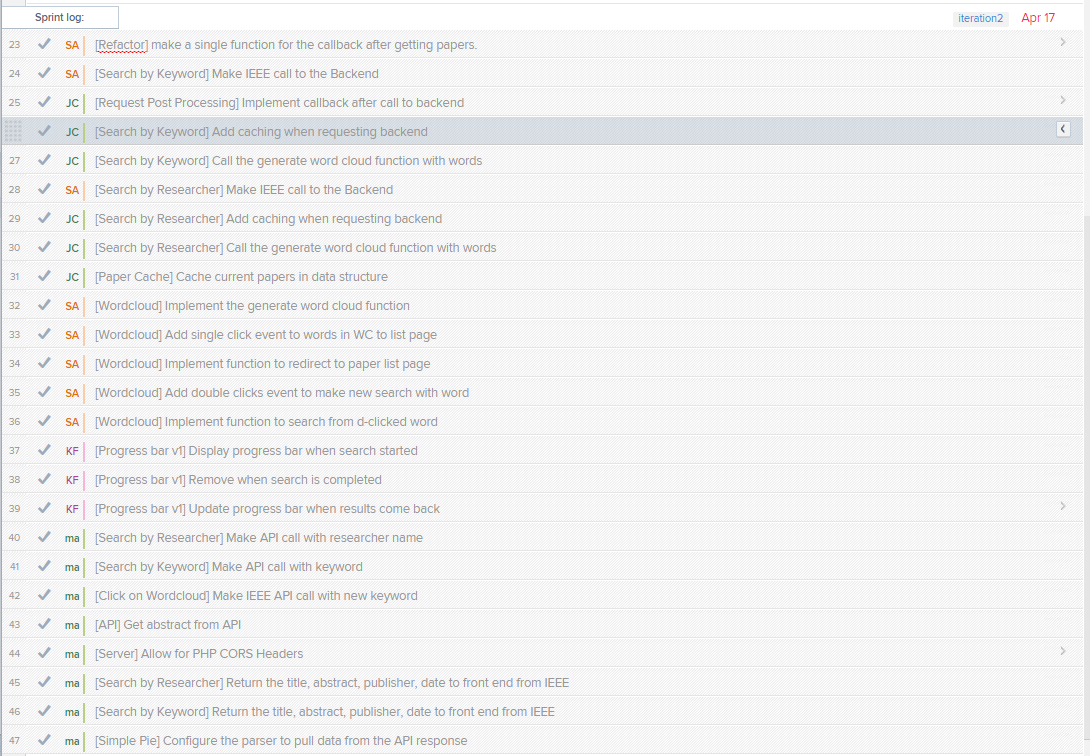
\includegraphics{images/sprintlog.png}
\caption{The Sprintlog for Iteration 2}
\end{figure}


\subsection{2.3 Meetings}\label{meetings}


\begin{figure}[htbp]
\centering
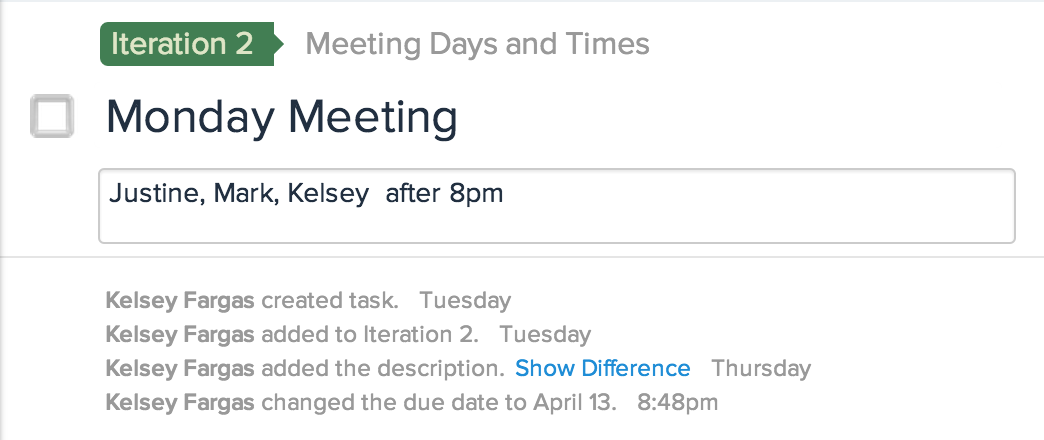
\includegraphics{images/meeting_example.png}
\caption{An example of meeting}
\end{figure}

Our team had a sprint planning meeting on Sunday April 5th in which we
set up various future group meeting times for the weeks of our
implementation phase. These meeting times are documented in Asana. All
team members then signed up to participate in four to five meetings
based on their availabilities. In this process, we were able to have
rotating teams to allow for variance in our pair programming practices
while keeping in line with having the team meet every day. If members of
the team could not meet in person, we had set up meetings that would be
online to continue our daily meeting schedule.


\begin{figure}[htbp]
\centering
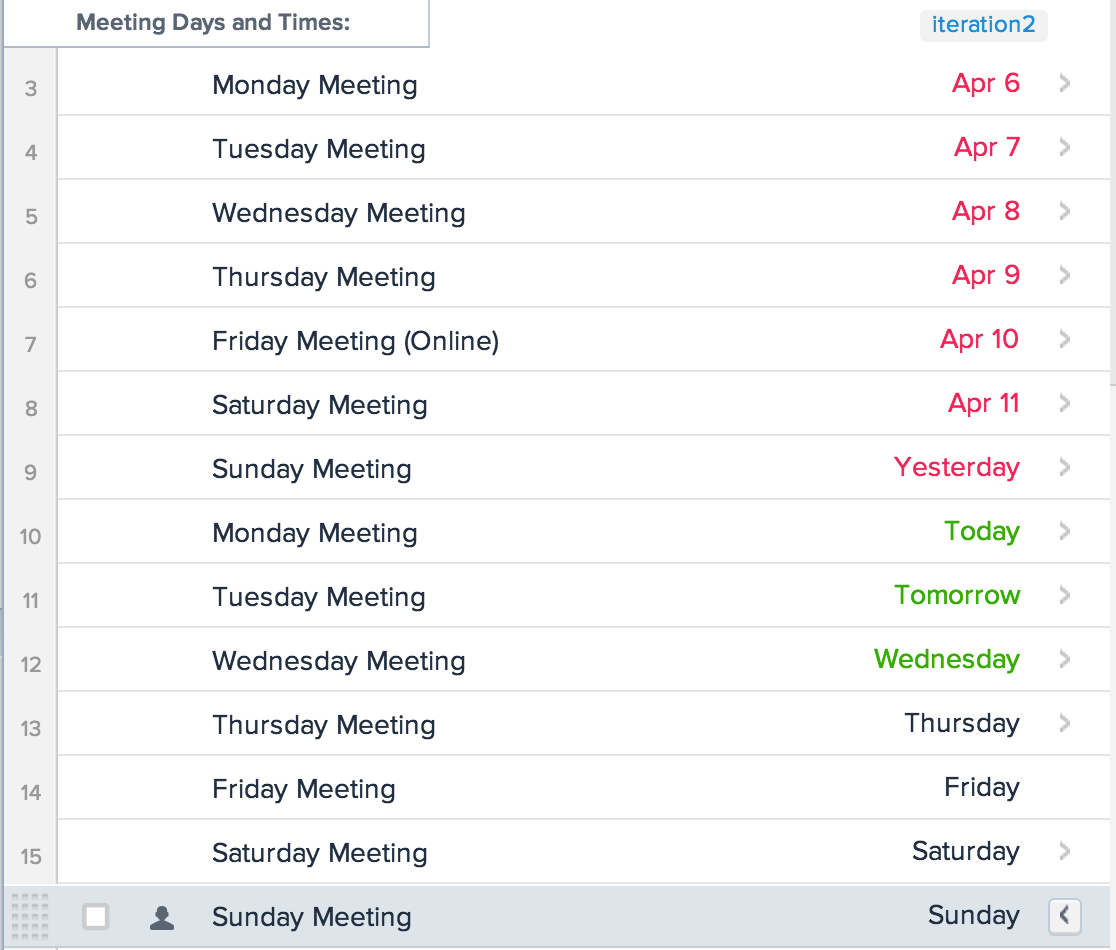
\includegraphics{images/meeting_dates.png}
\caption{The list of the meeting dates}
\end{figure}

\section{3 Extreme Programming
Practices}\label{extreme-programming-practices}

Extreme programming (XP) is an agile software engineering methodology
which enforces several practices. It is a natural companion to the SCRUM
process, as both of them are iterative and organized in sprints.

In addition to extending Agile practices to the extreme, XP also
promotes its own values and assumptions. The values include:

\begin{itemize}
\itemsep1pt\parskip0pt\parsep0pt
\item
  \textbf{Communication}: Communication is essential for adjusting to
  feedback and implementing constant changes. Honest, regular
  communication should not only happen amongst developers, but also
  amongst their customers.
\item
  \textbf{Feedback}: Feedback is the response from the customer to
  clarify what is required and wanted. By asking questions and making
  adjustments accordingly, the development team will be able to ensure
  that the code complies with the customer's specifications.
\item
  \textbf{Simplicity}: The development team should only focus on what
  really needs to be built and only solve the current problems of the
  day.
\item
  \textbf{Courage}: In this case, courage means making difficult
  decisions when necessary. It could be easy to disregard an issue
  because addressing it would make several people unhappy. Courage
  implies speaking up and pointing out difficulties.
\end{itemize}

Extreme programming not only assumes that each stakeholder will
incorporate the mentioned values, but also makes the following
assumptions:

\begin{itemize}
\itemsep1pt\parskip0pt\parsep0pt
\item
  \textbf{Enough Time and Resources}: Instead of rushing through the
  coding process, XP enables developers to work at their normal paces.
  By working in very short cycles, it reduces the length of time between
  actions and their effects. It also adjusts the project to fit the
  available resources.
\item
  \textbf{Constant Cost of Change}: XP ensures a constant change of
  cost. This means that implementing a functionality now versus in a
  year will take the same amount of effort. By making this assumption,
  it allows developers to focus on current tasks without worrying about
  future features.
\item
  \textbf{Developper Effectiveness}: Extreme programming assumes that in
  order to have great software, the developers should be great as well.
\item
  \textbf{Freedom to Experiment}: Every team member (including managers,
  developers, and customers) should have the opportunity to experiment.
  This means asking question such as ``Is there a better way to solve
  this problem ?'' and keeping an open mind towards the answers.
\end{itemize}

\subsection{3.1 Coding Practices}\label{coding-practices}

\subsubsection{3.1.1 Simple Code and
Design}\label{simple-code-and-design}

Simple code and design were practiced to make our code more efficient
and straightforward. The development started by defining what frameworks
to use and choosing the ones that are most flexible with respect to
change of direction for long term purposes. AngularJS and Slim were
chosen for this reason. The development team also implemented features
using libraries and reused code, taking out unnecessary functionalities
when needed. This is shown in the comparison of code from C-Lyrics - the
team's previous project - and PaperCloud, as well as the use of
jqcloud2. Another example of following the simple code and design was in
the implementation of the backend; we did not even check if our approach
was compatible with ACM's digital library and only focused on IEEE.

\subsubsection{3.1.2 Refactor Mercilessly}\label{refactor-mercilessly}

\begin{figure}[htbp]
\centering
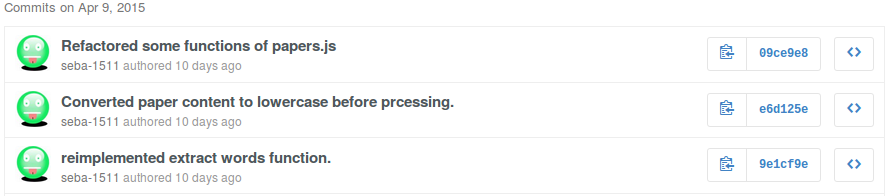
\includegraphics{images/refactor_commits.png}
\caption{Example of commits for refactoring}
\end{figure}

The purpose of refactoring is to have better, more readable as well as
more efficient code. This is a crucial step in order to obtain readable
code and reduce the cost of change. The developing team refactored their
code as soon as changes were needed or repetitions could be avoided. The
goal was to improve code's readability, document some of the main
functions, and remove superficial or unused functionalities. Refactoring
can be seen all along the git log commits. 

\begin{figure}[htbp]
\centering
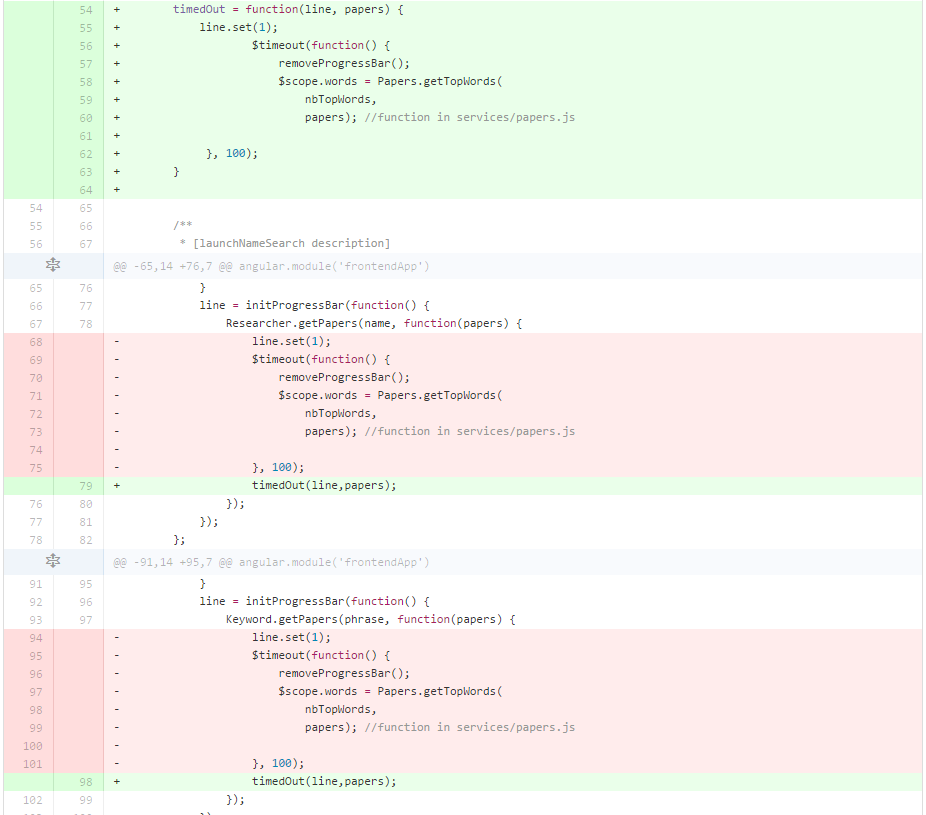
\includegraphics{images/refactor.png}
\caption{Diff of a refactoring commit}
\end{figure}


\subsubsection{3.1.3 Coding Standards}\label{coding-standards}

Coding standards are required to enable readability and communication
through code. By having everyone writing code in the same manner, the
team ensures that any developer will have some degree of familiarity
with the whole codebase. The developers used custom code formatting
templates to ensure homogeneity over the entire code. The code is openly
available on GitHub as mentioned in Section 1.6, and the formatting
templates are available at https://github.com/seba-1511/st\_settings.

Specifically we agreed to follow the JavaScript AirBnB guidelines
(available at: https://github.com/airbnb/javascript) but slightly
customized them to fit our team better. For example, we tried whenever
possible to keep all variable declarations at the beginning of a
function, and to minimize the number of var statements. For both PHP and
JavaScript, we used the DocBlocker plugin for SublimeText 2 in order to
keep the same amount of information between both ends.

\begin{figure}[htbp]
\centering
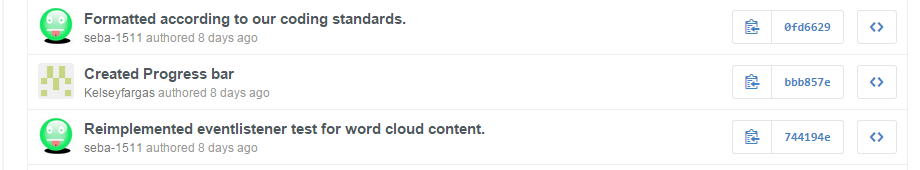
\includegraphics{images/kelsey_pair.png}
\caption{Refactoring to respect coding standards}
\end{figure}


\subsubsection{3.1.4 Common Metaphor}\label{common-metaphor}

The idea behind having a common metaphor is to describe the project as
it evolves. It allows the development team to share a vocabulary that
will define well-understood relationships. For this project, the
development team used a previous project as a metaphor. While not being
the most creative, this was highly useful as every team member was able
to clearly visualize the different parts of the application and how they
related to each other. The specific project was the creation of a lyrics
retrieval website which offered a lot of similar functionalities to the
current project.

\subsection{3.2 Developer Practices}\label{developer-practices}

\subsubsection{3.2.1 Test Driven
Development}\label{test-driven-development}

\begin{figure}[htbp]
\centering
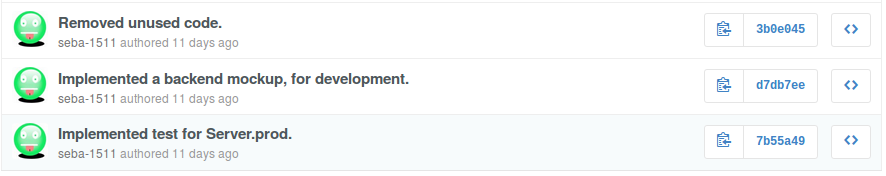
\includegraphics{images/test_driven.png}
\caption{First the test, then the implementation}
\end{figure}

Before implementing any functionality, we first wrote unit tests for
functional requirements or end-to-end tests for visual requirements.
This practice is underlined in our GitHub commit history. Due to the
absence of a customer in our team, we do not consider these tests as
acceptance tests. However, the visual tests were developed using the
same framework and methodology that the customer would be using for
acceptance testing.


\subsubsection{3.2.2 Pair Programming}\label{pair-programming}

\begin{figure}[htbp]
\centering
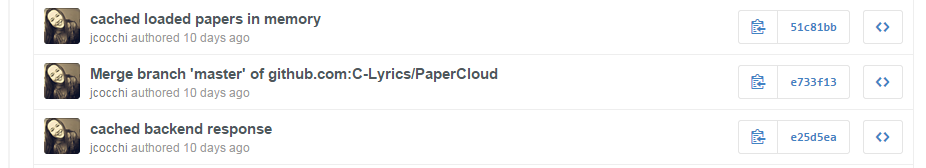
\includegraphics{images/justine_pair.png}
\caption{Commits of Justine and Sébastien pair programming}
\end{figure}

Pair programming is the process of programming in pairs with separate
roles: driver and observer. The driver writes code actively, while the
observer passively guides and discusses the code being written with the
driver. During all of our team meetings, we made sure that at least two
team members were engaging in pair programming. This practice provides
two significant benefits: uniformization of code throughout the project
and collective code ownership.

\subsubsection{3.2.3 Collective Code
Ownership}\label{collective-code-ownership}

\begin{figure}[htbp]
\centering
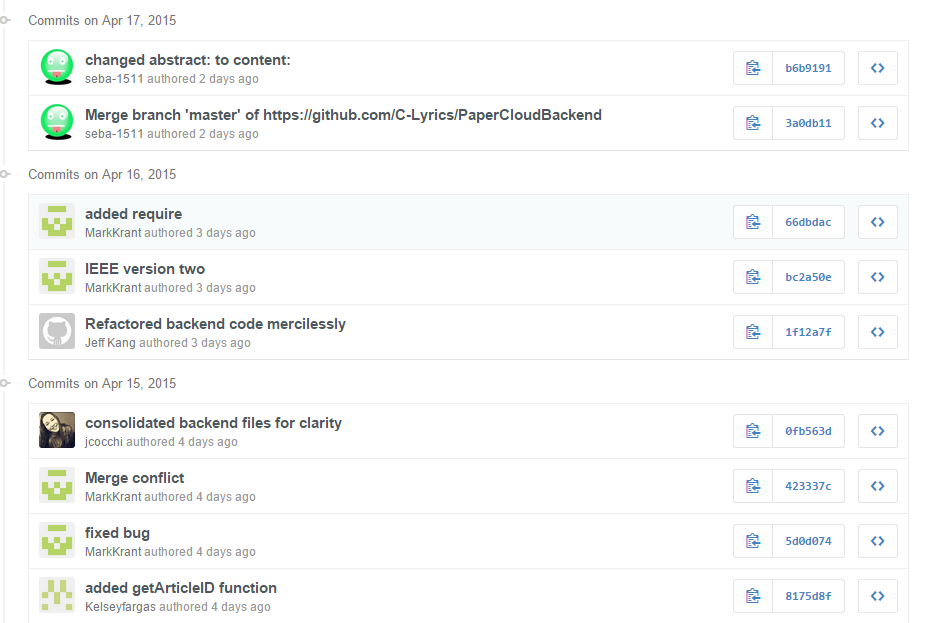
\includegraphics{images/code_ownership.png}
\caption{The whole team pushed to the repositories}
\end{figure}

Collective code ownership was created by having all members of the
development team commit to both the frontend and backend repositories.
This means that all team members are partially responsible for all
aspects of the final product. Following this practice ensured that
steady progress could be made on the project despite some team members
being absent each meeting, and it also helped to create a more cohesive
team dynamic.

In particular we followed this methodology by allowing access to both
repositories to all team members and avoiding restrictions on what
developers should work on. In order to take advantage of the strengths
of each team members, we also matched experienced ones to pair program
with novice ones. The result was that every team member felt comfortable
with every part of the program, despite not necessarily being an expert
about it.

\subsubsection{3.2.4 Continuous Integration and
Testing}\label{continuous-integration-and-testing}

\begin{figure}[htbp]
\centering
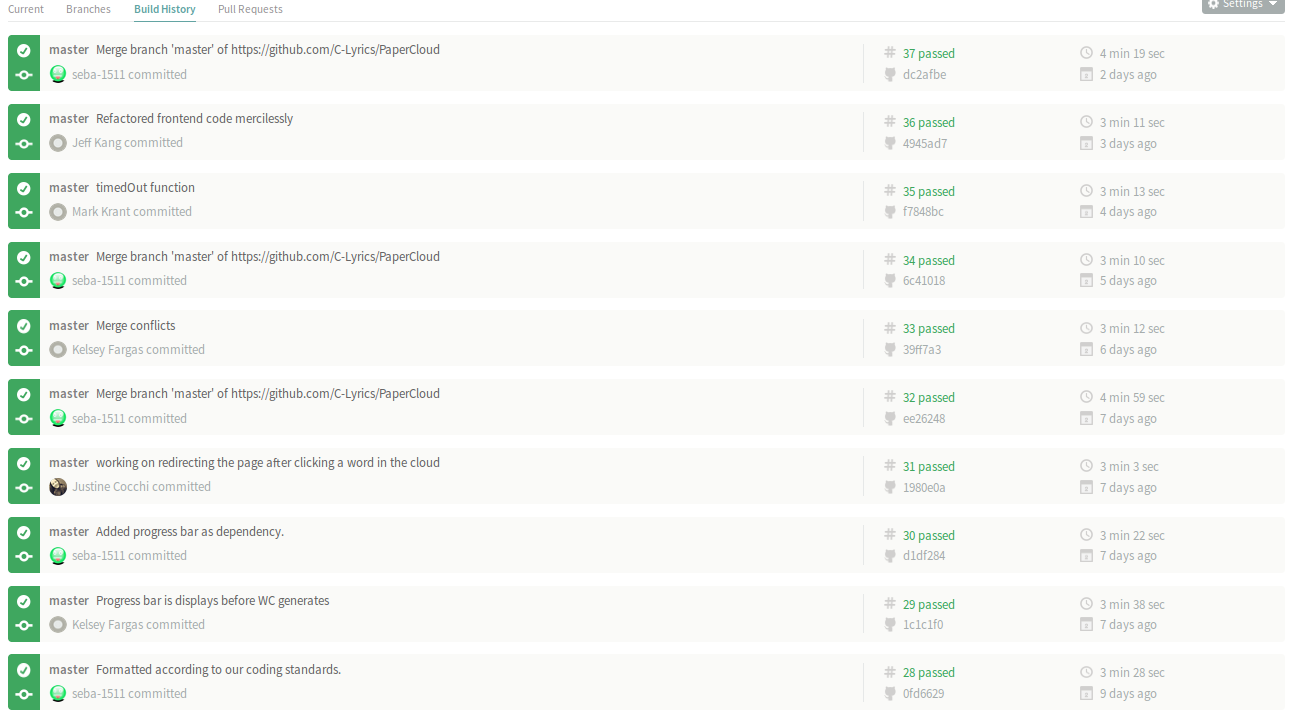
\includegraphics{images/travis_history.png}
\caption{Travis-CI build and test history}
\end{figure}

To apply continuous integration, our team set up a GitHub account and
TravisCI. This allowed us to consistently make sure that we all shared
the same code base, and it allowed us to monitor which commits broke our
tests. Those tests are mostly unit and acceptance tests, and a minor
part of them is testing the integration. That is because both backend
and frontend are completely independent, and they only require a
predefined API structure.

By using TravisCI we also automated the execution of tests across
repositories. As a matter of fact the provided service is to run all
tests of a given codebase as soon as a new version has been pushed to
the repository. A list of all executed tests can be found below, as is
one example of the resulting report.

\begin{figure}[htbp]
\centering
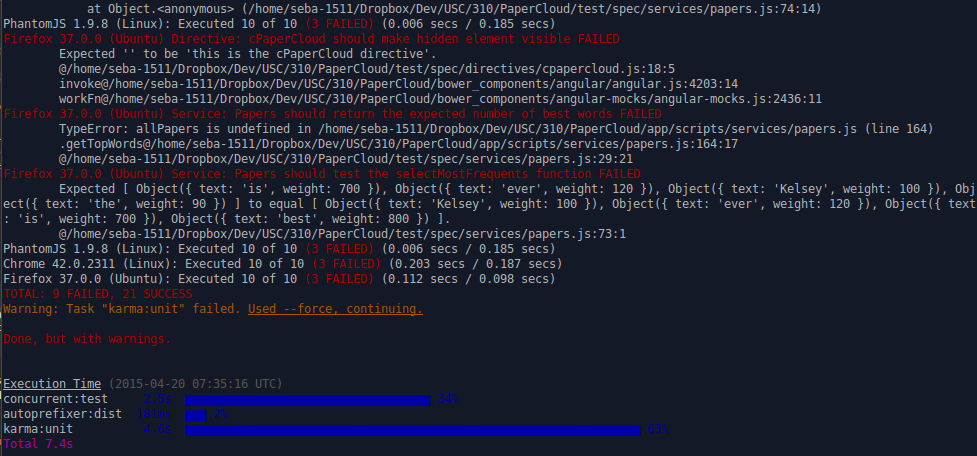
\includegraphics{images/test_output.png}
\caption{Example of testing output}
\end{figure}

\subsection{3.3 Business Practices}\label{business-practices}

\subsubsection{3.3.1 Customer Team Member}\label{customer-team-member}


\begin{figure}[htbp]
\centering
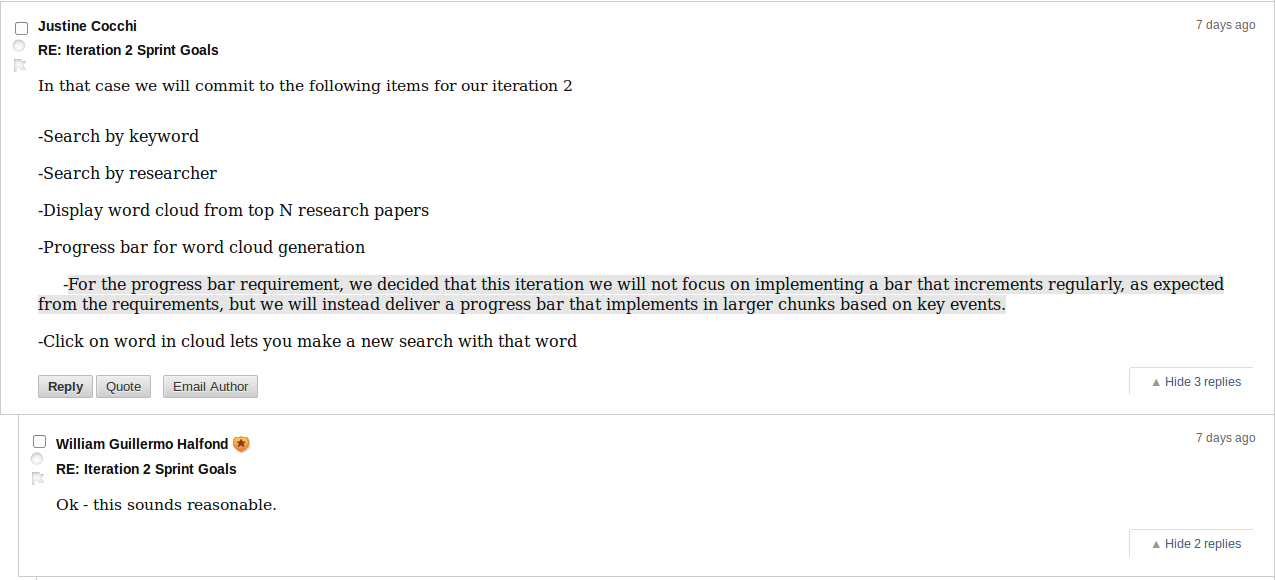
\includegraphics{images/conv_client.png}
\caption{A conversation with the client}
\end{figure}

One of the main obstacles of adhering to Extreme programming practices
was that it was not possible to have the customer as a team member due
to the special circumstances of the project being completed in a class
environment. Instead of working closely with the customer during our
meetings, the team focused on separate meetings with the customer and
inferred preferences from conversations through Blackboard and in-person
meetings. 

\subsubsection{3.3.3 Regular Releases}\label{regular-releases}

After this first iteration, the team can now submit a fully working and
tested system. This will hopefully be the case for next iterations,
which will allow for regular releases. As outlined in the iteration
review, we overestimated our capacities with respect to our sprint log.
However, after the final refactoring, the requirements we decided to
tackle are fully completed, and modifying the implemented functions will
only occur if new functionalities are to be added that conflict with
pre-existing functionalities.

\subsubsection{3.3.4 Sustainable Pace}\label{sustainable-pace}

\begin{figure}[htbp]
\centering
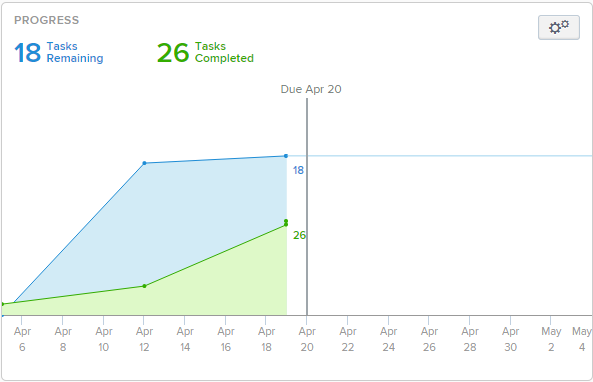
\includegraphics{images/burndown.png}
\caption{Our special "burnup" chart}
\end{figure}

The team held meetings every day during this sprint for an average time
of 2 hours each meeting. Because of this, we did not necessarily have to
``rush'' or overwork ourselves. This is represented in GitHub's
contribution graph in the figure below, which proves our steady pace. By
superimposing both contributions graph, we obtain an almost constant one
proving that we did work on very steady pace for the whole sprint.

In addition, the burndown chart - which is actually a burnup chart -
shows that we were able to make constant progress over the span of the
sprint. A note of caution with this chart: it includes all tasks related
to the sprint, including notes and meeting times. As we did not ``check
them off'' for practical purposes, it might seem like the sprint log
tasks were not completed whereas we actually finished all of them.

\begin{figure}[htbp]
\centering
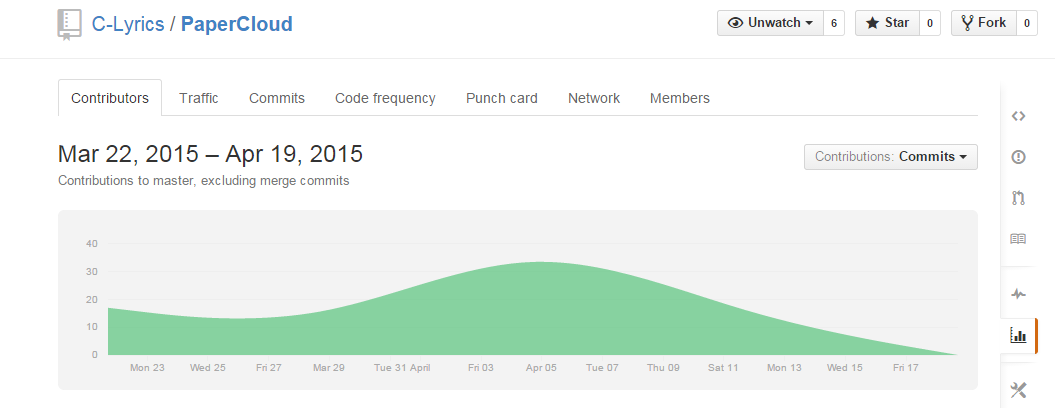
\includegraphics{images/contributions_front.png}
\caption{Summary of contributions to the frontend repository}
\end{figure}

\begin{figure}[htbp]
\centering
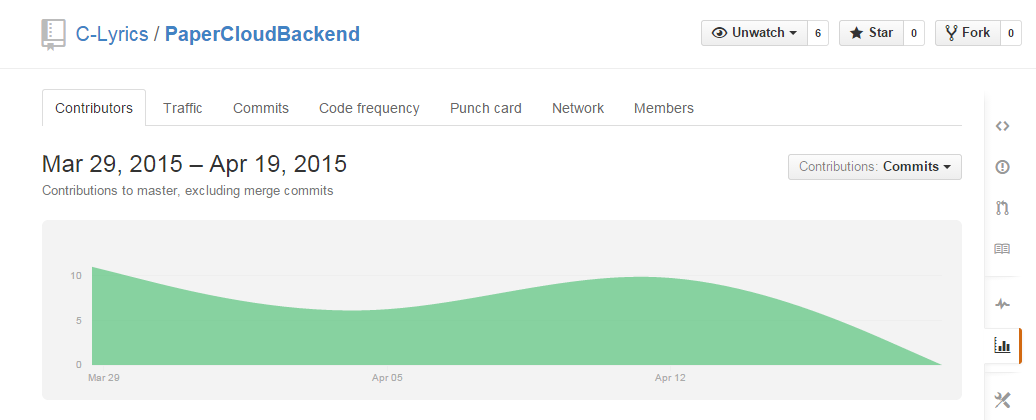
\includegraphics{images/contributions_back.png}
\caption{Summary of contributions to the backend repository}
\end{figure}

\subsection{4 Artifacts}\label{artifacts}

\subsubsection{4.1 Story Cards}\label{story-cards}

Although the customer was not involved with writing the story cards as
required by the official process, the following cards have been created
from the project requirements addressed in this iteration. If story
cards were used as a strategy for requirements engineering, the customer
would have arranged these in order of importance for prioritization.

Users should be able to search by keyword for articles Users should be
able to search by researcher name for articles A wordcloud should appear
after a search has been completed Clicking on a word in the wordcloud
should perform a new search with that keyword A progress bar should show
what progress is of the word cloud being generated

\subsubsection{4.2 The Bullpen}\label{the-bullpen}

In order to simulate an effective bullpen, our team booked rooms in
Leavey library for our meetings. In accordance with bullpen strategies,
these rooms are isolated, and team members have laptop computers to move
around freely and engage in pair programming. We were not, however, able
to have the customer in the room with us to ask clarifying questions.

\section{5 Iteration Review}\label{iteration-review}

\subsection{5.1 Sprint Review}\label{sprint-review}

Our sprint review took place at a meeting on April 17th with two
development team members present as well as the customer. We discussed
the completed items on our product and sprint backlogs, aspects of our
project that need improvement to add to the product backlog for the next
sprint, and the timeline for future progress with this project.

\subsubsection{5.1.1 Completed Product Backlog
Items}\label{completed-product-backlog-items}

Below is a list of completed product backlog items. We implemented an
extra item from the backlog that we had not originally committed to on
our sprint backlog in section 2.2.3, click on word in cloud lets you see
all research papers with that word in it and how frequently the word
appears in each one, because we had extra time during the sprint.

\begin{itemize}
\itemsep1pt\parskip0pt\parsep0pt
\item
  Search by keyword (IEEE publications only)
\item
  Search by researcher (IEEE publications only)
\item
  Display word cloud with common words from top N pages (user can't pick
  N)
\item
  Progress bar for progress of generating word cloud (large increments,
  not smooth progress)
\item
  Click on word in cloud lets you make new search with that word
\item
  Click on word in cloud lets you see all research papers with that word
  in it and how frequently the word appears in each one
\end{itemize}

\subsubsection{5.1.2 Completed Sprint Backlog
Items}\label{completed-sprint-backlog-items}

Below is a list of completed sprint backlog items, including items that
were added during the sprint because we had extra time. We were able to
complete all items from our sprint backlog.

\begin{itemize}
\itemsep1pt\parskip0pt\parsep0pt
\item
  Search by Researcher (IEEE publications only)

  \begin{itemize}
  \itemsep1pt\parskip0pt\parsep0pt
  \item
    Implement researcher search function
  \item
    Make API call with researcher name
  \item
    Parse PDF's with PHP
  \item
    Get the abstract from IEEE API
  \end{itemize}
\item
  Search by keyword (IEEE publications only)

  \begin{itemize}
  \itemsep1pt\parskip0pt\parsep0pt
  \item
    Implement keyword search function
  \item
    Make API call with keyword
  \item
    Parse PDF's with PHP
  \item
    Get the abstract from IEEE API
  \end{itemize}
\item
  Display word cloud from top N research papers

  \begin{itemize}
  \itemsep1pt\parskip0pt\parsep0pt
  \item
    Implement the generate WC function
  \end{itemize}
\item
  Progress bar for word cloud generation

  \begin{itemize}
  \itemsep1pt\parskip0pt\parsep0pt
  \item
    Display progress bar when search started
  \item
    Update when results come back
  \item
    Removed when search is completed
  \end{itemize}
\item
  Click on word in cloud lets you make new search with that word

  \begin{itemize}
  \itemsep1pt\parskip0pt\parsep0pt
  \item
    Implement double click event to make a new search with the word
  \item
    Implement function to search from double clicked word
  \end{itemize}
\item
  Click on word in cloud lets you see all research papers with that word
  in it and how frequently the word appears in each one

  \begin{itemize}
  \itemsep1pt\parskip0pt\parsep0pt
  \item
    Implement single click event to words in WC
  \item
    Implement function to redirect to paper list
  \end{itemize}
\end{itemize}

\subsubsection{5.1.3 Timeline}\label{timeline}

Based on the current state of the product backlog, the development team
is ahead of schedule. They were able to not only finish their sprint
backlog, but also complete an item that was not initially committed to.
Next sprint, the development team plans to continue adding functionality
to the system and fix the errors that were pointed out by the customer
during the sprint review.

\subsubsection{5.1.4 Customer Feedback}\label{customer-feedback}

Below is a list of feedback the customer gave the development team
during the sprint review.

\begin{itemize}
\itemsep1pt\parskip0pt\parsep0pt
\item
  The whole page should fit on the screen without having to scroll down
  to see the bottom
\item
  There is a little dash underneath the line that spans the top of the
  page that should be removed
\item
  Progress bar should update linearly rather than in large chunks as it
  does now
\item
  User is unable to make a second search without refreshing the page
\item
  After pressing the home button the user is not able to make a new
  search
\item
  The progress bar does not show up when making a new search from a word
  in the cloud by double clicking it
\item
  A high priority task for next iteration is adding functionality to the
  listing page of researchers including being able to go to the link to
  download the paper and having the information for each paper formatted
  properly
\item
  Word cloud itself is not very pretty and seems to only have two sizes
  and colors instead of a broader range
\item
  Add navigation buttons to go from the listing page back to the word
  cloud page
\end{itemize}

\subsection{5.2 Sprint Retrospective}\label{sprint-retrospective}

The development team's sprint retrospective took place at a development
team meeting on April 19th at 6:00pm with all members present.

\subsubsection{5.2.1 Identify What Went
Well}\label{identify-what-went-well}

The development team was successfully able to have at least three
members meet every day. This allowed the development team to make steady
progress towards completion of this sprint's goal. The team worked well
together and was able to split up jobs based on each team member's
strengths to optimize time. Additionally, everyone worked on both the
back end and front end for better understanding of the program and
collective code ownership. This sprint, the development team adhered to
more XP practices and was consequently much more efficient in completing
sprint backlog items.

\subsubsection{5.2.2 Identify What Needs
Improvement}\label{identify-what-needs-improvement}

The development team will focus on writing better acceptance and
integration tests to improve both next sprint's process and its product.
While the team got a lot more backlog items done this sprint than the
last sprint, the quality of some of the completed work was low. As
mentioned in section 5.1.4, the customer found many faults with the
implemented product and fixing them will be a top priority for the next
sprint, alongside implementing new functionality.

\subsubsection{5.2.3 Plan to Improve Process Next
Sprint}\label{plan-to-improve-process-next-sprint}

The development team plans to continue test driven development to
increase the quality of the delivered product. Instead of writing a
couple tests to satisfy the requirement of doing tests first, the team
will focus on writing useful tests that will help to catch errors, even
if that means spending more time on testing. This will create the
possibility of being able to complete as many backlog items as were
completed during this sprint, but the team feels that quality of the
work is more important than completing a large quantity of requirements.

\subsection{5.3 Scrum Meetings Review}\label{scrum-meetings-review}

All scrum meeting minutes can be found with timestamps on the online
blackboard forum for team 6 in the ``Iteration 2 Team Activity Log''
thread. Additionally, all of the meeting minutes are listed in the
Appendix in section 6.1 for the stakeholders' convenience.

\subsection{5.4 Customer Integration
Review}\label{customer-integration-review}

The development team met with the customer, Professor William G.
Halfond, to ensure that neither the priority for the requirements nor
the requirements themselves had changed for the project. The development
team used this information to build the updated product backlog and then
select items to move to this sprint's backlog. The sprint backlog was
checked with the customers to ensure that they agree that the decided
tasks were reasonable for this sprint.

Ideally, the team would have met with both Professor Halfond and Sonal
Mahajan to verify requirements and check progress throughout the sprint,
but Sonal was unavailable to meet. To make up for this, the team posted
some questions and clarifications on the Blackboard thread to ensure
that Sonal could give input as well as Professor Halfond.

In addition to several meetings during the sprint, the development team
also met with Professor Halfond for the sprint review, as documented in
full in section 5.1 and all of its subsections.

\section{6 Appendices}\label{appendices}

\subsection{6.1 SCRUM Meeting Minutes}\label{scrum-meeting-minutes}

\begin{itemize}
\itemsep1pt\parskip0pt\parsep0pt
\item
  Iteration 2: Scrum Meeting 1, April 8, 2015 (6:30pm - 7:45pm)

  \begin{itemize}
  \itemsep1pt\parskip0pt\parsep0pt
  \item
    Seb

    \begin{itemize}
    \itemsep1pt\parskip0pt\parsep0pt
    \item
      Q1: Last time we set the meeting times.
    \item
      Q2: I will work on integrating the several parts of the
      application together. Specifically, I want to have the word cloud
      displayed with mock-up data.
    \item
      Q3: No problem as of right now, everything is rocking.
    \end{itemize}
  \item
    Kelsey

    \begin{itemize}
    \itemsep1pt\parskip0pt\parsep0pt
    \item
      Q1: Last time I worked on setting meeting times.
    \item
      Q2: I will work on refactoring code, completing functions, and
      adding mock up code for testing functionality. Specifically, I
      will work on the function that assigns links to the words in the
      word cloud.
    \item
      Q3: I am still becoming more familiar with the code and the way it
      is organized.
    \end{itemize}
  \item
    Mark

    \begin{itemize}
    \itemsep1pt\parskip0pt\parsep0pt
    \item
      Q1: Last time I worked on setting meeting times.
    \item
      Q2: This time I will be working on making the back end compatible
      with the front end.
    \item
      Q3: I have problems with the simple pie parser, but I will resolve
      it soon.
    \end{itemize}
  \end{itemize}
\item
  Iteration 2: Scrum Meeting 2, April 9, 2015 (6:30pm - 9:00pm)

  \begin{itemize}
  \itemsep1pt\parskip0pt\parsep0pt
  \item
    Seb

    \begin{itemize}
    \itemsep1pt\parskip0pt\parsep0pt
    \item
      Q1: Last time I integrating the several parts of the application
      together.
    \item
      Q2: This time, I will work on post processing the request to the
      back end and pair programming for paper caching with Justine.
    \item
      Q3: The problems is that regular expression is difficult to do
      well.
    \end{itemize}
  \item
    Kelsey

    \begin{itemize}
    \itemsep1pt\parskip0pt\parsep0pt
    \item
      Q1: Last time I worked on refactoring code, completing functions,
      and adding mock up code for testing functionality
    \item
      Q2: This time, I will work on creating a progress bar and having
      it show up.
    \item
      Q3: I am having problems with creating and integrating the
      progress bar.
    \end{itemize}
  \item
    Mark

    \begin{itemize}
    \itemsep1pt\parskip0pt\parsep0pt
    \item
      Q1: Last time I worked on making the back end compatible with the
      front end.
    \item
      Q2: This time I work on searching by title for the back end.
    \item
      Q3: I am still having problems with the simple pie parser.
    \end{itemize}
  \item
    Justine

    \begin{itemize}
    \itemsep1pt\parskip0pt\parsep0pt
    \item
      Q1: Last time I helped make the schedule and the sprint backlog in
      the sprint planning meeting
    \item
      Q2: This time I am working on paper caching and pair programming
      with Seb.
    \item
      Q3: No problems yet.
    \end{itemize}
  \end{itemize}
\item
  Iteration 2: Scrum Meeting 3, April 10, 2015 (3:30pm - 5:00pm)
  {[}Note: This meeting was held over the phone as opposed to previous
  meetings which were all in person{]}

  \begin{itemize}
  \itemsep1pt\parskip0pt\parsep0pt
  \item
    Seb

    \begin{itemize}
    \itemsep1pt\parskip0pt\parsep0pt
    \item
      Q1: Last time I worked with Justine and implemented a caching DS
      for papers with its tests, I tested and implemented the post
      processing of the response from the backend, and got a first nice
      visualization to work.
    \item
      Q2: Today I will test and implement click events on the word
      cloud's words.
    \item
      Q3: Angular has a directive for clicks and double clicks, so
      everything is chill.
    \end{itemize}
  \item
    Justine

    \begin{itemize}
    \itemsep1pt\parskip0pt\parsep0pt
    \item
      Q1: Last time I pair programed with Seb to implement caching the
      papers and the corresponding tests for that.
    \item
      Q2: This time I will research how to implement the progress bar.
    \item
      Q3: No problems yet.
    \end{itemize}
  \end{itemize}
\item
  Iteration 2: Scrum Meeting 4, April 11, 2015 (9:00am - 12:30pm)

  \begin{itemize}
  \itemsep1pt\parskip0pt\parsep0pt
  \item
    Seb

    \begin{itemize}
    \itemsep1pt\parskip0pt\parsep0pt
    \item
      Q1: Tried to implement click and double click function but it was
      not working.
    \item
      Q2: Today I fixed some of the problems with the click and double
      click function and will continue fixing them. Pair program with
      Kelsey to complete progress bar.
    \item
      Q3: Stuck on code above, the jqcloud doesn't support passing
      events to directives
    \end{itemize}
  \item
    Kelsey

    \begin{itemize}
    \itemsep1pt\parskip0pt\parsep0pt
    \item
      Q1: Last time I worked on having a progress bar show up in the
      main page.
    \item
      Q2: This time, I will work on removing the progress bar and
      creating tests for the progress bar.
    \item
      Q3: I am having problems with finding ways to remove the progress
      bar.
    \end{itemize}
  \item
    Milad

    \begin{itemize}
    \itemsep1pt\parskip0pt\parsep0pt
    \item
      Q1: Last time I was learning the technologies to use for
      development
    \item
      Q2: I will start coding this week, all set up now.
    \item
      Q3: Lacking fundamental understanding of the why and how the tools
      we are using are helpful or different. Not detrimental, but I can
      be more efficient when I get it.
    \end{itemize}
  \end{itemize}
\item
  Iteration 2: Scrum Meeting 5, April 12, 2015 (9:00am - 12:30pm)

  \begin{itemize}
  \itemsep1pt\parskip0pt\parsep0pt
  \item
    Seb

    \begin{itemize}
    \itemsep1pt\parskip0pt\parsep0pt
    \item
      Q1: Last time I tried to fix some of the problems with the click
      and double click function and will continue fixing them. Pair
      program with Kelsey to complete progress bar.
    \item
      Q2: Today I will write test for the listening page and implement a
      mock up of the listing page.
    \item
      Q3: No problems as of right now.
    \end{itemize}
  \item
    Kelsey

    \begin{itemize}
    \itemsep1pt\parskip0pt\parsep0pt
    \item
      Q1: Last time I worked on removing the progress bar and created
      tests for it.
    \item
      Q2: This time, I will work on implementing the double click
      function for the word cloud.
    \item
      Q3: I am having problems with checking if the double click
      function works. Will keep testing.
    \end{itemize}
  \item
    Justine

    \begin{itemize}
    \itemsep1pt\parskip0pt\parsep0pt
    \item
      Q1: Last time I researched how to implement the progress bar.
    \item
      Q2: This time, I will work on implementing the function to
      redirect to paper list page.
    \item
      Q3: I am having problems with redirecting the listing the page
      from the word cloud.
    \end{itemize}
  \item
    Jeff

    \begin{itemize}
    \itemsep1pt\parskip0pt\parsep0pt
    \item
      Q1: Last time I helped with the meeting times and schedule.
    \item
      Q2: This time, I will pair program with Kelsey.
    \item
      Q3: I have no problems.
    \end{itemize}
  \item
    Milad

    \begin{itemize}
    \itemsep1pt\parskip0pt\parsep0pt
    \item
      Q1: Last time I was learning the technologies to use for
      development.
    \item
      Q2: This time, I will work on getting the environment setup.
    \item
      Q3: I am having problem installing bower packages.
    \end{itemize}
  \end{itemize}
\item
  Iteration 2: Scrum Meeting 6, April 13, 2015 (8:00:pm-9:00pm)

  \begin{itemize}
  \itemsep1pt\parskip0pt\parsep0pt
  \item
    Kelsey

    \begin{itemize}
    \itemsep1pt\parskip0pt\parsep0pt
    \item
      Q1: Last time I worked on implementing the double click function
      for the word cloud.
    \item
      Q2: This time, I will work on the documentation process.
    \item
      Q3: I am not having any problems
    \end{itemize}
  \item
    Justine

    \begin{itemize}
    \itemsep1pt\parskip0pt\parsep0pt
    \item
      Q1: Last time I worked on implementing the function to redirect to
      paper list page.
    \item
      Q2: This time, I will work on the documentation process.
    \item
      Q3: I do not have any problems.
    \end{itemize}
  \item
    Mark

    \begin{itemize}
    \itemsep1pt\parskip0pt\parsep0pt
    \item
      Q1: I refactored some of the arxiv API code to meet new demands
      specified by Sebastien.
    \item
      Q2: Working on integrating the IEEE api into the back end to
      access other documents.
    \item
      Q3: No problem so far with IEEE, the api seems very functional,
      but still unsure on how to access ACM digital library.
    \end{itemize}
  \end{itemize}
\item
  Iteration 2: Scrum Meeting 7, April 14, 2015 (9:00am - 12:30pm)

  \begin{itemize}
  \itemsep1pt\parskip0pt\parsep0pt
  \item
    Seb

    \begin{itemize}
    \itemsep1pt\parskip0pt\parsep0pt
    \item
      Q1:Last time I wrote tests for the listing page.
    \item
      Q2: Today I will link the backend and the frontend with Mark, will
      try to fix the redirection to the listing page, and improve the
      display of the progressbar.
    \item
      Q3: Redirecting to the listing page is a funny business with
      Angular. I don't understand why it does not work, yet.
    \end{itemize}
  \item
    Mark

    \begin{itemize}
    \itemsep1pt\parskip0pt\parsep0pt
    \item
      Q1: I started parsing the IEEE API response.
    \item
      Q2: Today I will link the frontend with the backend with Seb. Then
      I will work on IEEE parsing and finish it, pair programming with
      Jeff.
    \item
      Q3: Linking the backend and the frontend might not be trivial.
    \end{itemize}
  \item
    Jeff

    \begin{itemize}
    \itemsep1pt\parskip0pt\parsep0pt
    \item
      Q1: Last time I got the environment setup.
    \item
      Q2: Today I will finish setting up my environment, and then pair
      program with Mark.
    \item
      Q3: Setting up the environment might be problematic.
    \end{itemize}
  \item
    Milad

    \begin{itemize}
    \itemsep1pt\parskip0pt\parsep0pt
    \item
      Q1: Last time I was setting up bower grunt and yo.
    \item
      Q2: This time, I will try to find the problem of why you can't
      make a second search.
    \item
      Q3: No problems, finally ready to implement stuff.
    \end{itemize}
  \end{itemize}
\item
  Iteration 2: Scrum Meeting 8, April 15, 2015 (6:00pm-8:00pm)

  \begin{itemize}
  \itemsep1pt\parskip0pt\parsep0pt
  \item
    Seb

    \begin{itemize}
    \itemsep1pt\parskip0pt\parsep0pt
    \item
      Q1:Last time I linked the backend and the frontend with Mark, will
      try to fix the redirection to the listing page, and improve the
      display of the progress bar.
    \item
      Q2: This time, I will work on a better progress bar.
    \item
      Q3: I have no problems so far.
    \end{itemize}
  \item
    Mark

    \begin{itemize}
    \itemsep1pt\parskip0pt\parsep0pt
    \item
      Q1: Last time, I linked the frontend with the backend with Seb.
      Then I will work on IEEE parsing and finish it, pair programming
      with Jeff.
    \item
      Q2: This time, I will continue to link the frontend with the
      backend.
    \item
      Q3: I have no problems so far.
    \end{itemize}
  \item
    Kelsey

    \begin{itemize}
    \itemsep1pt\parskip0pt\parsep0pt
    \item
      Q1: Last time I worked on updating the document for this
      iteration.
    \item
      Q2: This time, I will work on a getting method in backend for the
      articles ID.
    \item
      Q3: I am not having any problems.
    \end{itemize}
  \item
    Justine

    \begin{itemize}
    \itemsep1pt\parskip0pt\parsep0pt
    \item
      Q1: Last time I worked on updating the document for this
      iteration.
    \item
      Q2: This time, I will work on refactoring the backend.
    \item
      Q3: I do not have any problems.
    \end{itemize}
  \end{itemize}
\item
  Iteration 2: Scrum Meeting 9, April 16, 2015 (6:30pm-8:30pm)

  \begin{itemize}
  \itemsep1pt\parskip0pt\parsep0pt
  \item
    Mark

    \begin{itemize}
    \itemsep1pt\parskip0pt\parsep0pt
    \item
      Q1: Last time, I continued to link the frontend with the backend.
    \item
      Q2: This time, I am changing the back end to meet new requirements
      from the front end.
    \item
      Q3: I am having parsing problems.
    \end{itemize}
  \item
    Kelsey

    \begin{itemize}
    \itemsep1pt\parskip0pt\parsep0pt
    \item
      Q1: Last time I worked on a getting method in the backend for the
      articles ID.
    \item
      Q2: This time, I will work on the documentation.
    \item
      Q3: I am not having any problems.
    \end{itemize}
  \item
    Justine

    \begin{itemize}
    \itemsep1pt\parskip0pt\parsep0pt
    \item
      Q1: Last time I worked on refactoring the backend.
    \item
      Q2: This time, I will work on the documentation.
    \item
      Q3: I do not have any problems.
    \end{itemize}
  \item
    Jeff

    \begin{itemize}
    \itemsep1pt\parskip0pt\parsep0pt
    \item
      Q1: Last time I finished setting up my environment, and then pair
      programmed with Mark.
    \item
      Q2: This time, I will work on refactoring the front end and back
      end, and working on documentation.
    \item
      Q3: I do not have any problems.
    \end{itemize}
  \end{itemize}
\end{itemize}

\end{document}
